\section{Columnar Analysis Demonstrator}\label{sec:demonstrator}

One of the established research projects for columnar analysis is the development of an ATLAS columnar analysis demonstrator.
This demonstrator is inspired by the Institute for Research and Innovation in Software for High Energy Physics (IRIS-HEP)~\cite{S2I2HEPSP,CWPDOC} Analysis Grand Challenge~\cite{Held:2022sfw}, which leverages the ``PyHEP'' ecosystem of data science and analysis tools developed by IRIS-HEP and Scikit-HEP~\cite{Rodrigues:2020syo}.
These ecosystems of tools build upon and extend the broader Scientific Python ecosystem, with mature columnar analysis libraries, to provide functionality at each step of the columnar analysis pipeline: data query and access, data file I/O and columnar access, data transformation and histogramming, distributed analysis frameworks, statistical modelling and inference, and analysis reinterpretation.

The ATLAS Run 4 Analysis Model is built around the PHYSLITE common reduced data format~\cite{Schaarschmidt:2024vzr,SOFT-2022-02}.
PHYSLITE is a monolithic file format --- intended to support around 80\% of all physics analyses in Run 4 --- that contains already-calibrated physics objects for fast analysis, and allows for direct support without the need to create derived ROOT ntuples for analysis.
% The demonstrator uses ATLAS PHYSLITE open data~\cite{ATL-OREACH-PROC-2024-005,Marshall:2919097} --- released for research use for the first time in 2024 --- to ensure the accessibility and reproducibility of the technical demonstrator analysis.
The demonstrator uses ATLAS PHYSLITE open data~\cite{ATL-OREACH-PROC-2024-005} --- released for research use for the first time in 2024 --- to ensure the accessibility and reproducibility of the technical demonstrator analysis.
PHYSLITE has tight integration with ROOT features, to the extent that raw PHYSLITE is not easily loadable outside of ROOT in general.
Integrating PHYSLITE data access with the Python analysis ecosystem presents unique challenges, such as correctly handling ElementLinks and custom objects like triggers.
However, the Awkward Array~\cite{Awkward_Array_2018} library supports ``behaviors'' which allow for efficiently reinterpreting data structures on the fly, and can be used by Uproot~\cite{Uproot_2017} for I/O of custom serializations (e.g. PHYSLITE).
Through contributions by ATLAS members large amounts of PHYSLITE are now supported by both Uproot and Coffea~\cite{Coffea_2023,CMS:2020kpn} which allows for most workflows to proceed with small alterations.~\cite{US_ATLAS_IRISHEP_trainging:2024}
This allows for the demonstrator workflow to operate on most PHYSLITE files directly with Uproot, as seen in \Cref{fig:atlas-pipeline}, and for data in the PHYS ATLAS Run 3 Analysis Model data format~\cite{SOFT-2022-02}, FuncADL~\cite{funcadl_2024,Proffitt:2021wfh} and ServiceX~\cite{serviceX_2024,serviceX_client_2024,Galewsky:2020xig} can be used to create a distributed ROOT~\cite{Brun:1997pa} transformer to read the data and perform calibrations, producing an equivalent in-memory columnar representation as if the file had been PHYSLITE.
As PHYSLITE already contains all of the calibrated physics objects, it is preferable to use PHYSLITE whenever possible.

\begin{figure}
    \centering
    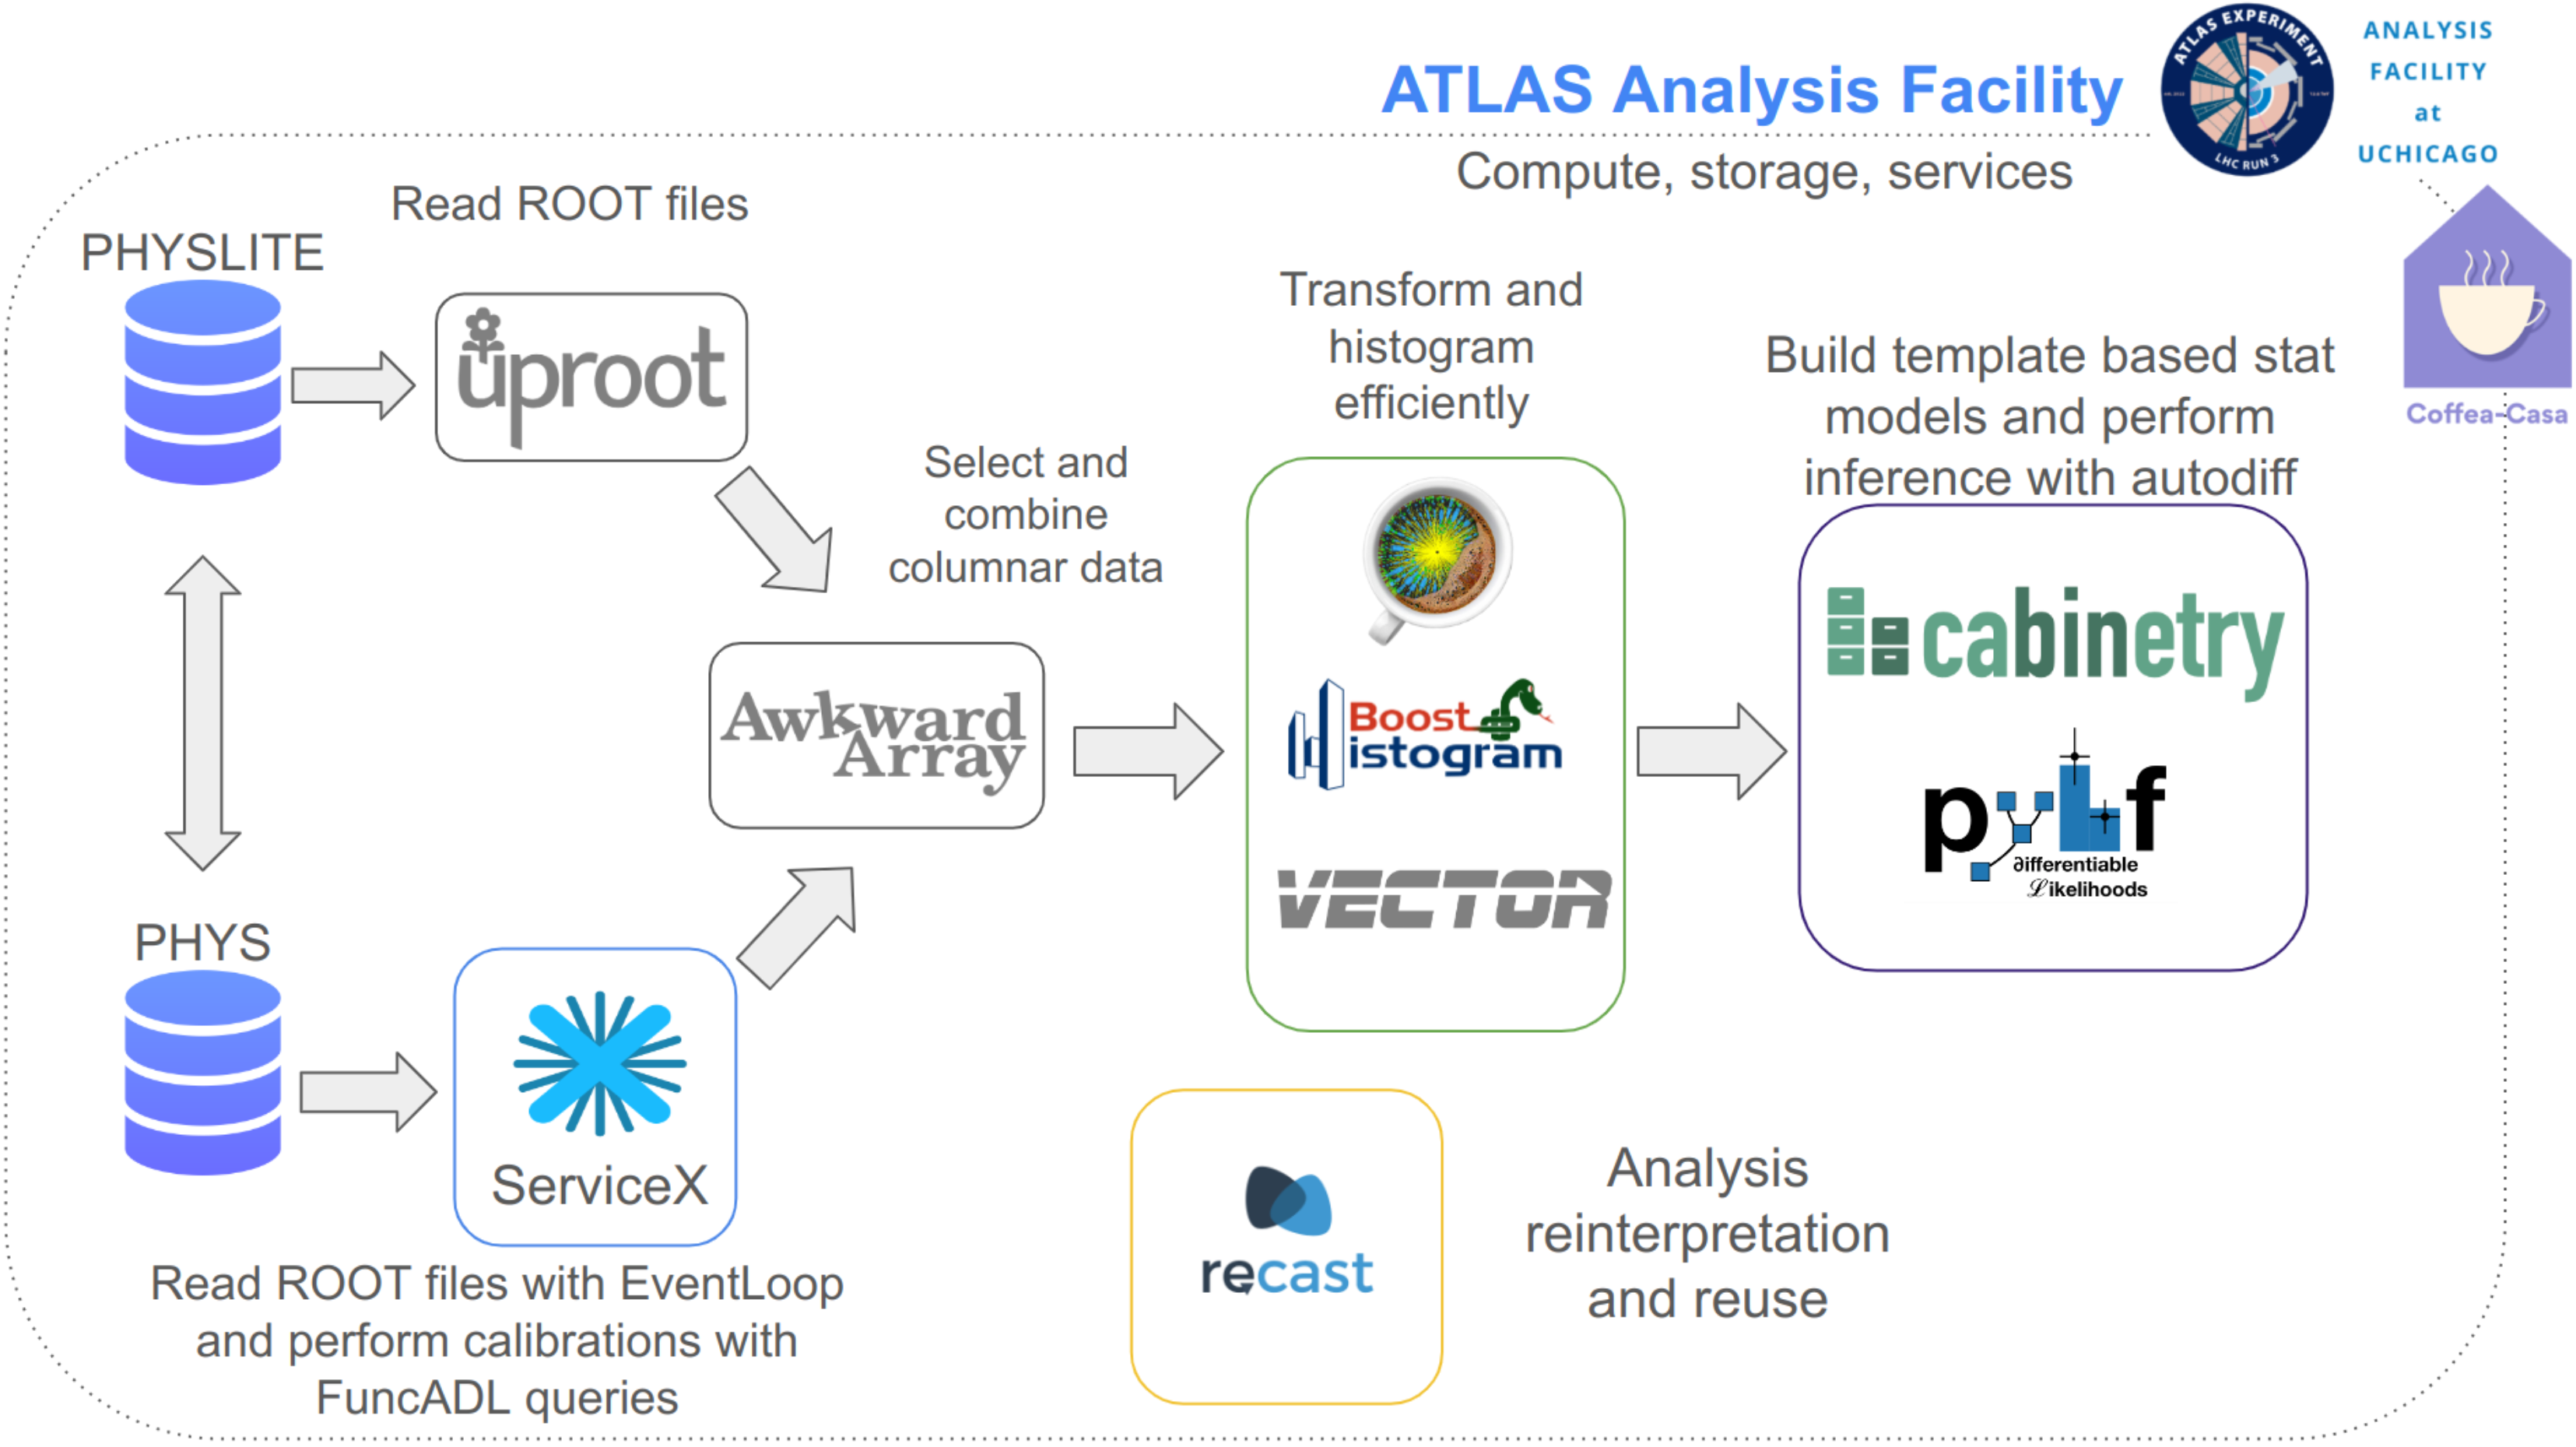
\includegraphics[width=\textwidth]{atlas-pipeline.png}
    \caption{Schematic outline of an ATLAS columnar analysis demonstrator able to operate on PHYS and PHYSLITE data formats using columnar analysis tools from the PyHEP ecosystem.
    The demonstrator is designed to be deployed and run at an ATLAS analysis facility, such as the University of Chicago Analysis Facility or a Coffea-casa deployment.}
    \label{fig:atlas-pipeline}
\end{figure}
